% This is a comment.
% the region directly below this comment, up till the command \begin{document} is known as the 'preamble'
% basic setup
\documentclass{article}
\usepackage[english]{babel}
\usepackage[utf8]{inputenc}

% for mathematics
\usepackage{amsmath}
\usepackage{amsthm}
% define theorems, lemmas, etc
\newtheorem{theorem}{Theorem}
\newtheorem{lemma}{Lemma}
\newtheorem{corollary}{Corollary}
\newtheorem{definition}{Definition}
\newtheorem{example}{Example}
\usepackage{amssymb}

% for adjusting margins
\usepackage{geometry}
\geometry{
	a4paper,
 	left=26mm,
 	right=20mm,
 	top=33mm,
 	bottom=38mm
}

% for introducing urls
\usepackage{url}

% for colored text
\usepackage{color}

% for creating lists
\usepackage{enumerate}

% for import graphics
\usepackage{graphicx}

% include algorithm package
\usepackage[]{algorithm2e}

% change font to times new roman
%\usepackage{times}

% title details
\title{QF4102 Financial Modelling and Computation Assignment 1}
%\date{}
\author{G01 Wang Zexin, Chen Penghao}

%~~~~~~~~~~~~~~~~~~~~~~~~~~~~~~~~~~~~~~~~~~~~~~~~~~~~~~~~~~~~~~~~~~~~~~~~~~~~~~
\begin{document}

% insert title
\maketitle
% make a new page
\newpage

\section{Question 1}
\subsection*{\emph{Statement of the problem}}
Write a Matlab function for the exact solution of a European down-and-out call option. Your function must be able to \textbf{work with the initial underlier price $S_{0}$ in a vector form}.
\subsection{Data collection and preparation}
The business day chosen, day X is 28 Feb, 2017 within the 9-day period. The settlement prices of Eurodollar futures contracts which expire in March 2017, June 2017, September 2017, December 2017, March 2018, \dots , up to December 2026, (i.e. 10 years into the future) have been collected from the CME group website into the \emph{raw\_data} sheet of the excel file.\\
A screenshot of the webpage has been obtained and shown below.
\begin{figure}[h]
  \centering
  \begin{minipage}[h]{0.32\textwidth}
    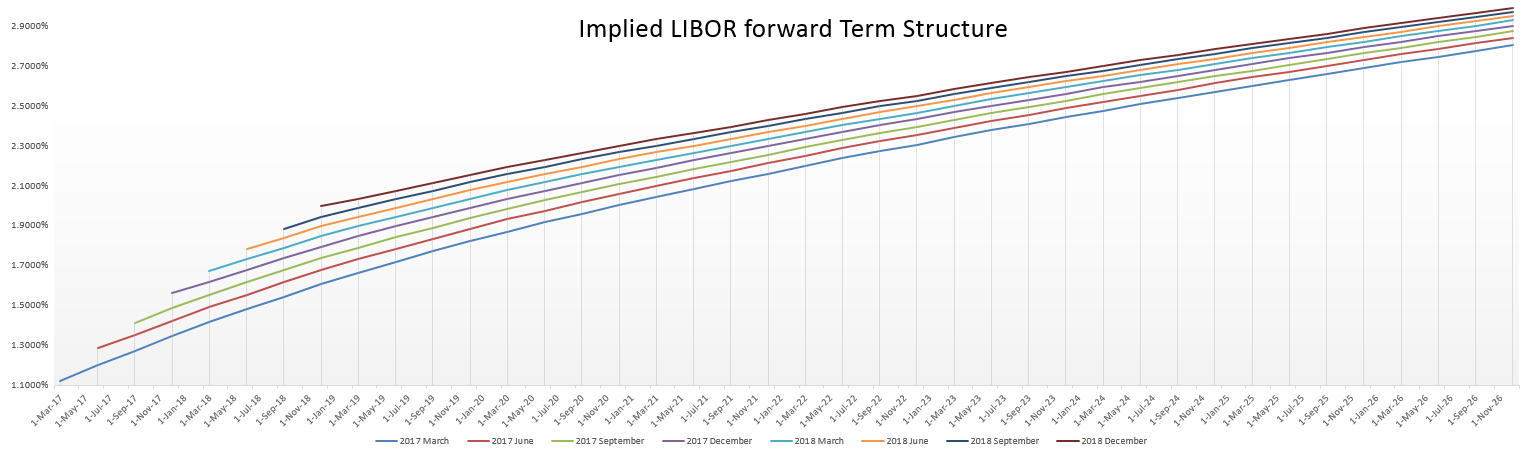
\includegraphics[width=\textwidth]{biu.PNG}
  \end{minipage}
  \hfill
  \begin{minipage}[h]{0.32\textwidth}
    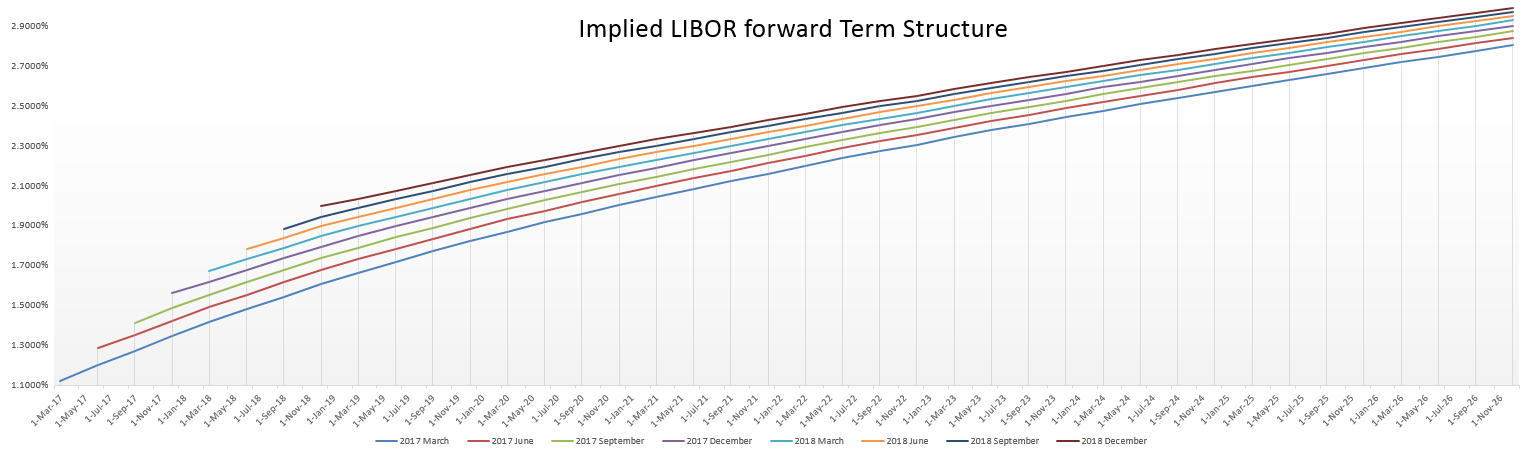
\includegraphics[width=\textwidth]{biu.PNG}
  \end{minipage}
  \hfill
  \begin{minipage}[h]{0.32\textwidth}
    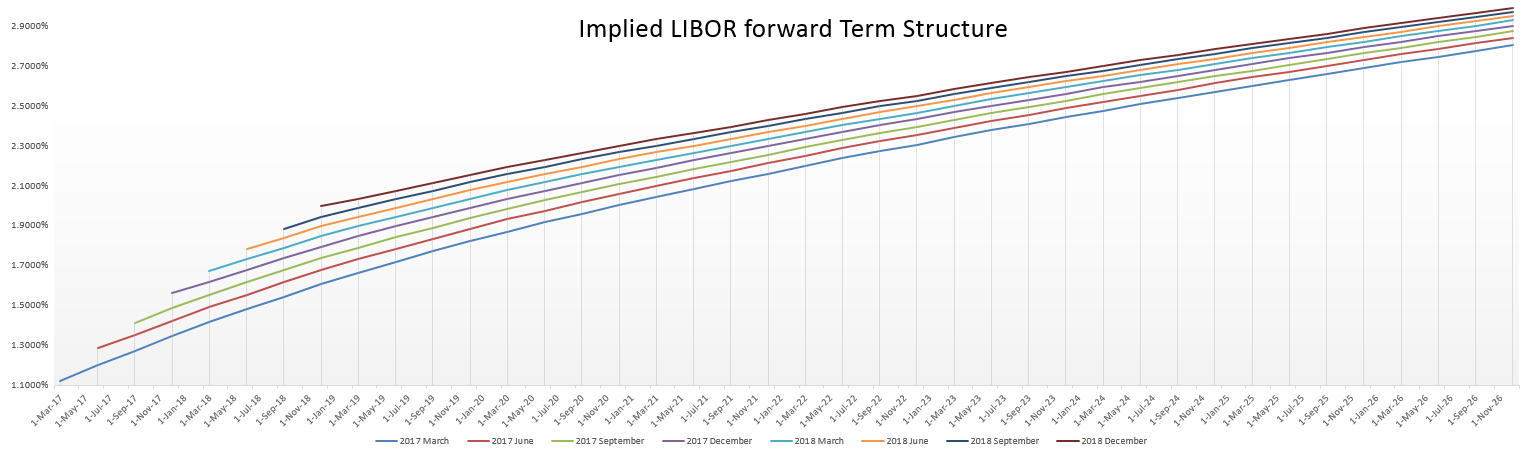
\includegraphics[width=\textwidth]{biu.PNG}
  \end{minipage}
	\caption{Screenshot of the webpage showing settlement prices of ED futures}
\end{figure}

Also, the expiry dates can be obtained from the CME group website. A sheet of the settlement dates have been collected into the \emph{raw\_dates} sheet of the excel file. A screenshot of the webpage has been obtained and shown below.
\begin{figure}[h]
	\centering
	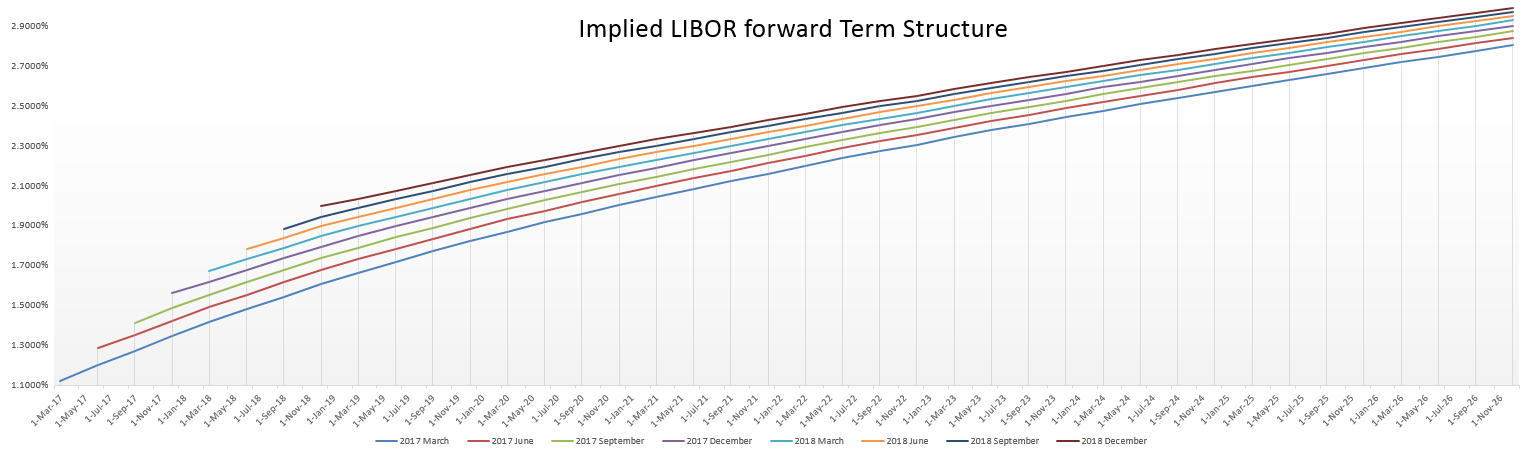
\includegraphics[scale=0.5]{biu.PNG}
	\caption{Screenshot of the webpage showing settlement dates of ED futures}
\end{figure}
\newpage

\subsection{Implied Forward LIBOR term structure}
As the index prices of Eurodollar futures have linear relationship with the implied forward 3-month LIBOR rate starting from the expiry dates of the Eurodollar futures until maturity of the Eurodollar time deposits, we are able to work out the implied forward 3-month LIBOR rates.\\[4mm]
Denote the forward rate from expiry date of the first futures to the $n$-th Eurodollar futures by $f_{n}$, numbers of days until maturity of the underlying of the $i$-th Eurodollar futures by $m_{i}$, implied 3-month LIBOR rate of the underlying of the $i$-th Eurodollar futures by $l_{i}$ and the settlement price of the $i$-th Eurodollar futures by $P_{i}$.\\[4mm]
$$1 + \frac{\sum_{i=1}^{n} m_{i}}{360}f_{n} = [\prod_{i=1}^{n} (1 + l_{i}\frac{m_{i}}{360}) - 1] \frac{\sum_{i=1}^{n} m_{i}}{360}$$
\begin{equation}
\begin{split}
f_{n} &= [\prod_{i=1}^{n} (1 + l_{i}\frac{m_{i}}{360}) - 1] \frac{360}{\sum_{i=1}^{n} m_{i}}\\
&= [\prod_{i=1}^{n} (1 + \frac{100 - P_{i}}{100}\frac{m_{i}}{360}) - 1] \frac{360}{\sum_{i=1}^{n} m_{i}}
\end{split}
\end{equation}
\\[4mm]Using equation (1), we are able to calculate the forward LIBOR rate to all the expiry dates of the Eurodollar futures. By applying the VBA cell-array function onto the settlement prices and dates data available, the term structure starting from March 2017 until December 2026 can be obtained. However, as the expiry date of the 2026 March Eurodollar futures is unknown yet, we have no clue how many days should we use for the last Eurodollar futures. Still I have used a dummy expiry date to mimic the expiry dates of the March contract in previous years. This may be a reasonable assumption given that the fluctuations of rates over a short time span of a few days are small, and that reference LIBORs are essentially averages from polling industrial players anyway.
\begin{figure}[h]
	\centering
	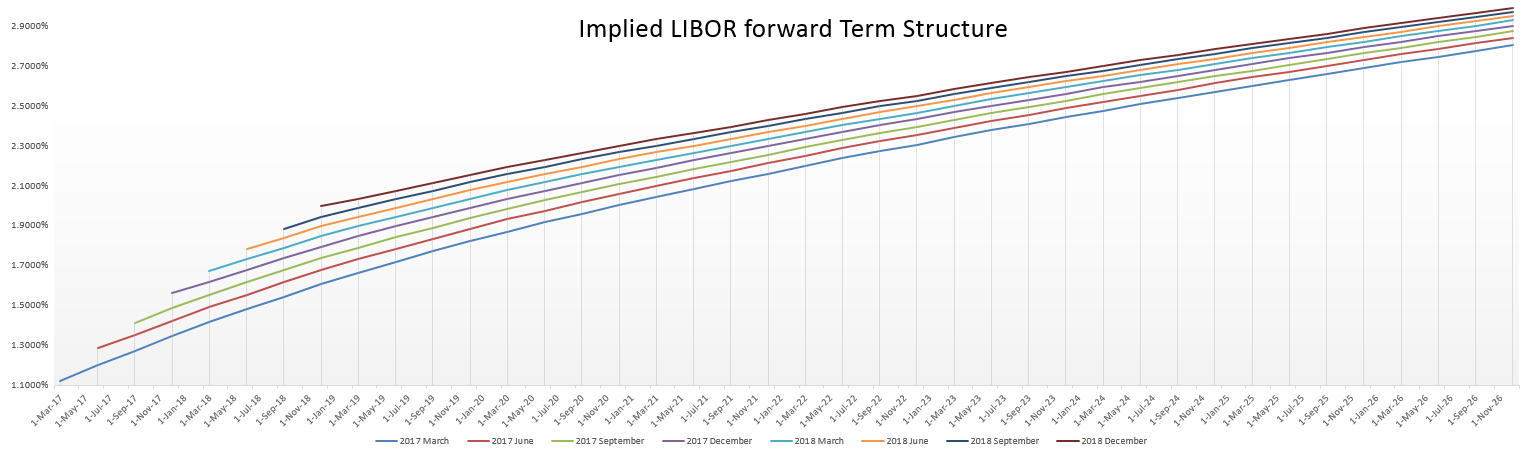
\includegraphics[scale=0.4]{biu.PNG}
	\caption{Implied Forward LIBOR Term Structure}
\end{figure}
\\[2mm]Above is a diagram plotted based on the Implied Forward LIBOR term structure. The diagram consists of 8 curves which stand for the forward rate term structure starting at March, June, September, December of 2017 and 2018. The diagram showed that the annualized forward rates are gradually increasing from $1.10\%$ to about $2.80\%$, over a time period from the beginning of 2017 to the end of 2026. There is one feature of this diagram that the term structures starting at different dates are of similar curvature, which is rational given that the 3-month LIBOR forward rates are gradually increasing. We can also see that the diagram has a convex curvature, which is reasonable as we expect to see the rate of change of the forward rates to decrease over time.
\newpage

\subsection{Swap Rate for Deferred Interest Rate Swap}
Similar to the previous section, we can work out forward term structure from the index prices of Eurodollar futures. The discount factors can be computed using the forward rates. The swap rate for deferred interest rate swap is simply the swap rate for the expected forward rates, as specified in equation (2).
\\Denote the discount factor from time 0 to $K$-th year by $d_{0,K}$, the forward rate (not annualized) from time 0 to the $i$-th year by $f_{i}$, and the swap rate by $r$.
\begin{equation}
\begin{split}
r &= \frac{1 - d_{0,K}}{\sum_{i=1}^{K} d_{0,i}}\\
&= \frac{1 - (1 + f_{K})^{-1}}{\sum_{i=1}^{K} (1 + f_{i})^{-1}}
\end{split}
\end{equation}
\\Tabulated series of deferred swap rates starting from the March, June, September and December of 2017 with maturity of 1, 2, \dots, 9 years are displayed in Figure 5:
\begin{figure}[h]
	\centering
	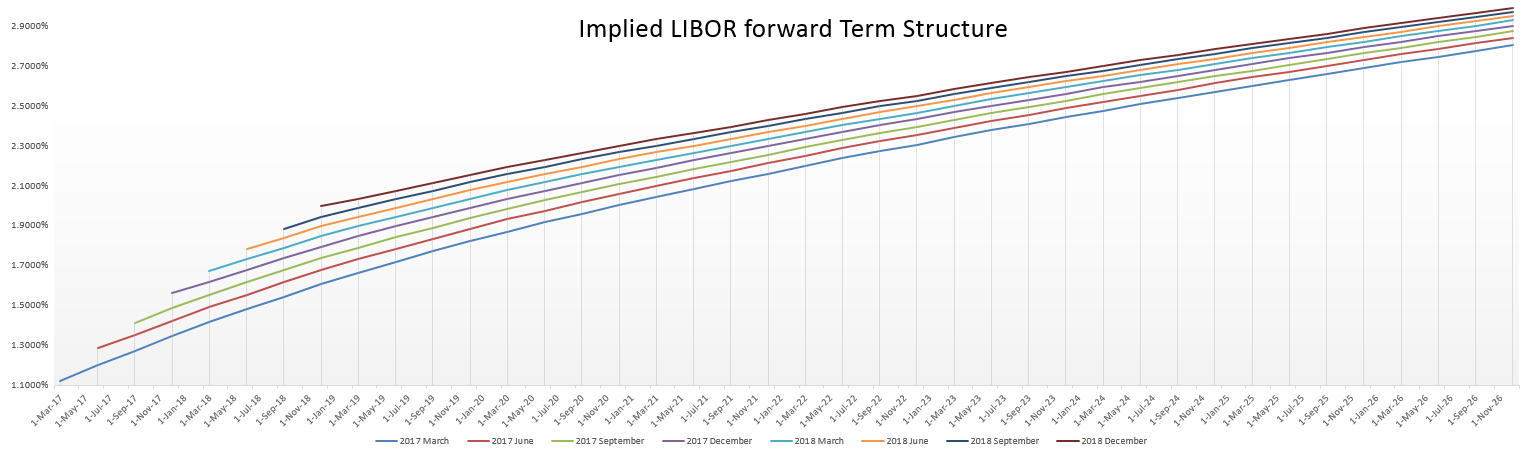
\includegraphics[scale=0.4]{biu.PNG}
	\caption{Deferred Interest Rate Swap Rate Table}
\end{figure}
\\Also, other than the illustrative use of the \emph{GetSwapRate} function in the excel sheets, the diagram of the deferred interest swap rates can be plotted.
\begin{figure}[h]
	\centering
	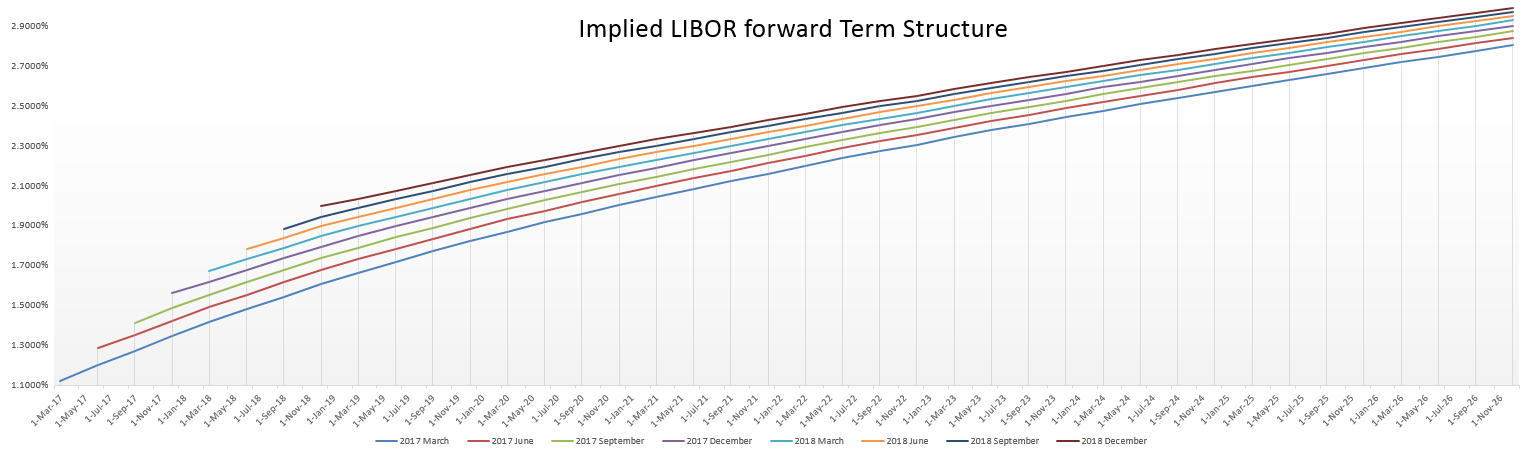
\includegraphics[scale=0.4]{biu.PNG}
	\caption{Deferred Interest Rate Swap Rates}
\end{figure}
\\We shall observe that the calculated deferred swap rates are rational, as the curvature of the upward curve is convex.
\newpage

\section{Efficient Stock Portfolios}
\subsection*{Statement of the problem}
Eight stocks of my choice, belonging to \textbf{differetn industrial or commercial sectors}, are to be selected for construction of efficient portfolios of these stocks.
\subsection{Data collection and preparation}
From \emph{http://finance.yahoo.com}, we can obtain the weekly stock price data within the time period of 5 years. The stocks I have chosen are from the industries Retail \& Hospitality, Energy, Financials, Healthcare, Business services, Computer software and services, Diversified Business, Manufacturing, and are respectively Amazon, Exxon Mobile, Goldman Sachs, Novartis AG, Fedex, Google, Berkshire Hathaway, Toyota Motor.\\[3mm]
The formula $r_{i} = \frac{v_{i}-v_{i-1}}{v_{i-1}}$ can be used to find the stock returns from the stock prices. The mean, sample covariance and sample variance functions which are built-in in excel are then applied onto the rates of return. An array of return rates and a covariance matrix are obtained as follows:
\begin{figure}[h]
  \centering
  \begin{minipage}[h]{0.85\textwidth}
    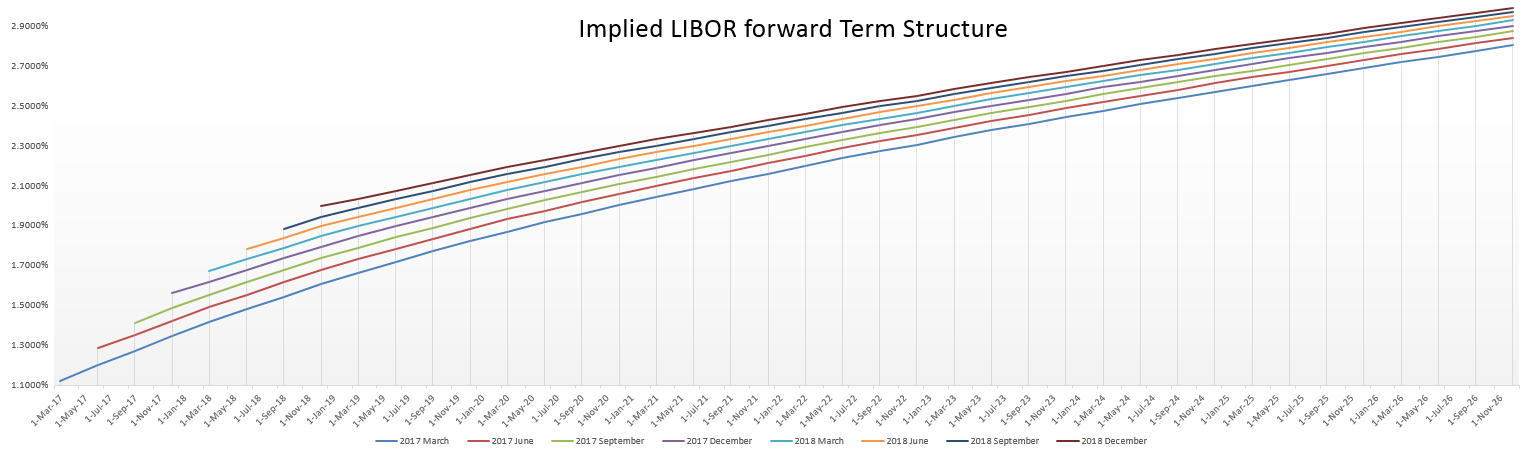
\includegraphics[width=\textwidth]{biu.PNG}
  \end{minipage}
  \hfill
  \begin{minipage}[h]{0.1\textwidth}
    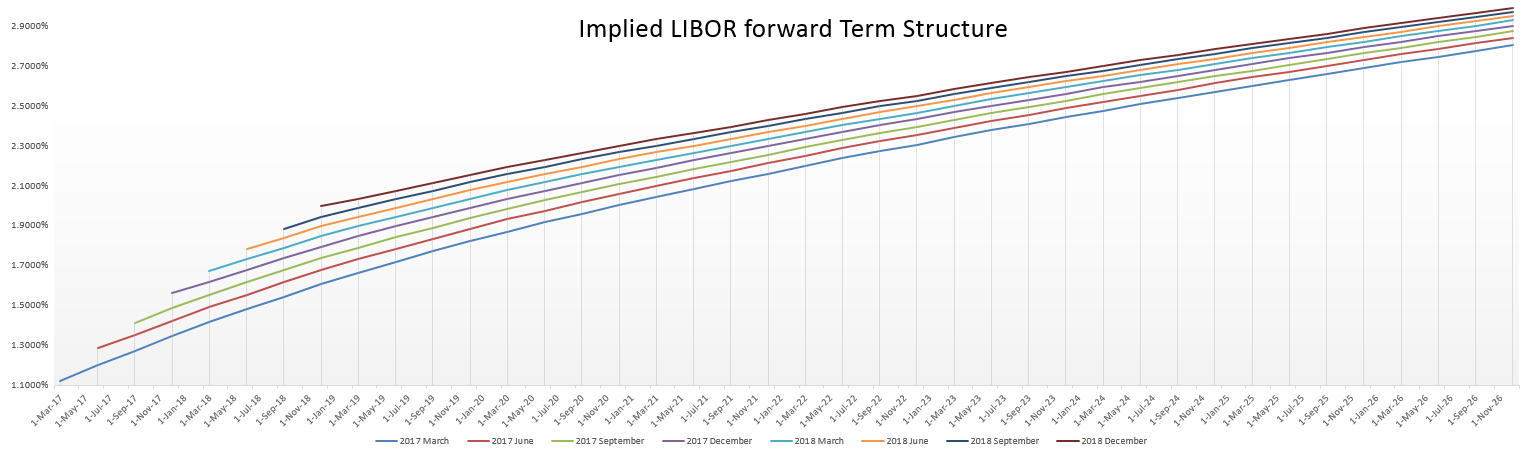
\includegraphics[width=\textwidth]{biu.PNG}
  \end{minipage}
  \caption{Covariance Matrix of the stock returns and Expected returns vector}
\end{figure}

\subsection{Newly issued European floating strike lookback put options}
Just like what we did in a previous tutorial, a minimum variance portfolio, or in short MVP, can be obtained from the covariance matrix directly by equation (3):
$$ \textbf{w}_{\text{MVP}} = \frac{\textbf{C}^{-1}\mathrm{1}}{\mathrm{1}^{T}\textbf{C}^{-1}\mathrm{1}} $$
\begin{equation}
\begin{split}
\textbf{w}_{i} &= \frac{\sum_{j=1}^{N} (\textbf{C}^{-1})_{i,j}}{\sum_{k=1}^{N}\sum_{j=1}^{N} (\textbf{C}^{-1})_{k,j}}
\end{split}
\end{equation}
\\[6mm]And an efficient portfolio weights can be calculated using equation (4) from the \textbf{Two-Fund Theorem}:
$$ \textbf{w}_{\text{efficient}} = \frac{\textbf{C}^{-1}\mathrm{\mu}}{\mathrm{1}^{T}\textbf{C}^{-1}\mathrm{\mu}} $$
\begin{equation}
\begin{split}
\textbf{w}_{i} &= \frac{\sum_{j=1}^{N} \mathrm{\mu}_{j}(\textbf{C}^{-1})_{i,j}}{\sum_{k=1}^{N}\sum_{j=1}^{N} \mathrm{\mu}_{j}(\textbf{C}^{-1})_{k,j}}
\end{split}
\end{equation}
As specified in the comments in the VBA functions, I have also checked for the number of rows and columns of the covariance matrix as well as the expected returns vector. If their dimensions do not match our expectations, a message box is used to inform the user. Assumption that the expected returns vector passed in is a column vector instead of a row vector has been made.
\newpage

\subsection{Not newly issued European floating strike lookback put options}
In the previous case we could take advantage of the characteristic of lookback option in which all the maximum values correspond to the potential stock prices in the binomial tree. However in this case, since the option is not newly issued and we may have a previous running max which does not correspond to any of the potential stock prices, we cannot use the single state variable to fully represent both the current stock price and the running max. Therefore the following adjustment is needed:
\begin{itemize}
	\item Compare $\tilde{A}$ and $S_{0}$, if $\tilde{A}$ is smaller, treat this like a newly issued lookback option and use the previous case's algorithm
	\item let $x_{0} = \ln \frac{\tilde{A}}{S_{0}}$
	\item Determine for an integer $j$ such that $j{^{\Delta}x} < x_{0} < (j+1){^{\Delta}x}$
	\item Grow two separate linear trees from $x_{0}^{j}$ and $x_{0}^{j+1}$
	\item Perform the backward time binomial updates
	\item Interpolate between two option values at the roots to obtain option premium
\end{itemize}
Below is an algorithm developed based on this idea:

\begin{algorithm}[H]
 \KwData{$r, \sigma, S_{0}, \tau, N, q, \tilde{A}$}
 \KwResult{$p_{0}$, Option Premium}
 Initialization\;
 let $\delta S = \frac{2S}{M}$ be the underlying asset price difference \;
 For stability, let $\delta t = \frac{0.9}{\sigma^{2}M^{2}}$ be the time difference\;
 $N = \frac{T}{\delta t}$\;
 We define the following vectors:\\
 $\alpha_{i} = \frac{1}{2}\delta t(\sigma^{2}i^{2} - ri), \beta_{i} = 1-\delta t(\sigma^{2}i^{2} + r), \gamma_{i} = \frac{1}{2}\delta t(\sigma^{2}i^{2} + ri), \forall \, 1 \le i \le M$\;
 Set the boundary conditions\;
 \For {i = 1 \dots M} {
  $V_{i, N} = f(i\,\delta S)$\;
 }
 \For {j = 1 \dots N} {
  $V_{M, j} = f(2S)e^{-r(N-j)\delta t}$\;
 }
 \For {j = N \dots 1} {
  \For {i = 2 \dots M-1} {
   $V_{i, j-1} = \sigma_{i}V_{i-1,j} + \beta_{i}V_{i,j} + \gamma_{i}V_{i+1,j} $\;
  }
 }
 $V_{\frac{M}{2},1}$ is the output value for option premium\;
\caption{One factor Explicit Euler scheme FDM algorithm}
\end{algorithm}
By adding up all the weights in one portfolio, we can do a quick check upon whether the normalization has been done correctly or not. As both of their weights add up to 1, we are certain that the normalization process has been done correctly. Checking upon other features of the expected returns and variances will be left to the graphing of efficient frontier.\\
After we have obtained the MVP and efficient portfolios, a convex set of 25 points can be computed based on different $\lambda$s assigned to the MVP and efficient portfolio. By the \textbf{Two-Fund Theorem}, we can use equation (5) to compute a series of portfolio weights on the efficient frontier when adjusting $\lambda$ from 0 to 1.
\begin{equation}
\begin{split}
\textbf{w}_{i} &= \lambda \textbf{w}_{\text{MVP}, i} + (1 - \lambda) \textbf{w}_{\text{efficient}, i}
\end{split}
\end{equation}
\begin{figure}[h]
	\centering
	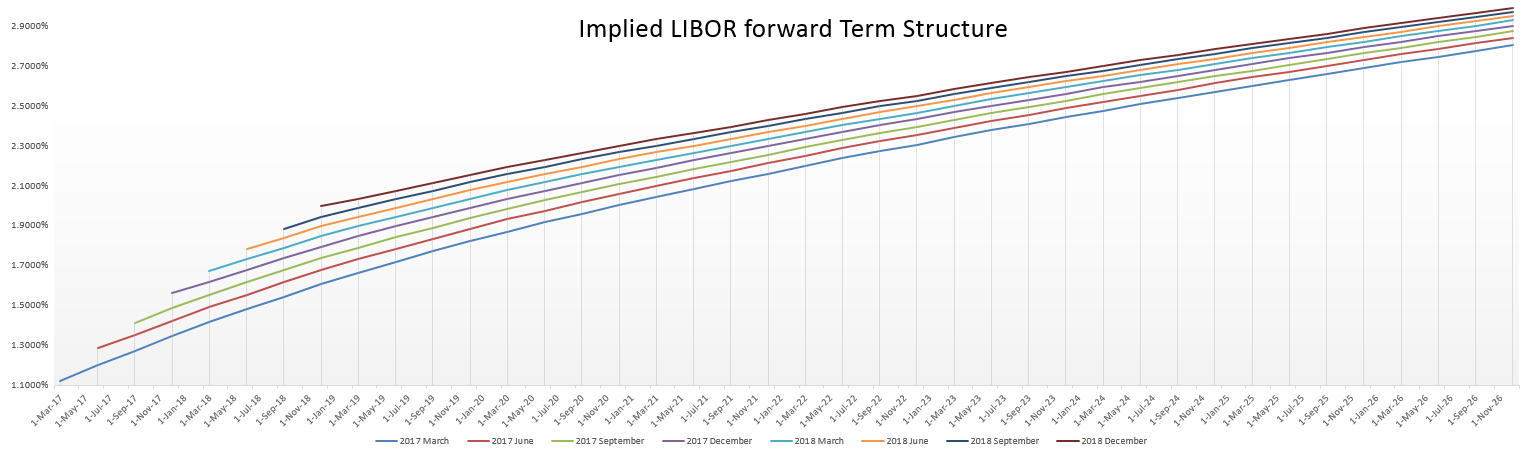
\includegraphics[scale=0.5]{biu.PNG}
	\caption{$\sigma-\bar{r}$ diagram of 25 points}
\end{figure}
\\From this $\sigma-\bar{r}$ diagram in Figure 8, since the expected return $\bar{r}$ is increasing with a convex curvature, this ensures that there will only be one capital market line going through the portfolios with the highest Sharpe ratio. Also, we can be certain that the expected return of the minimum variance portfolio is positive.
\newpage

\subsection{Analyze, compare and comment on the results}
From Figure 8, we can easily observe that the efficient portfolio has a much higher expected return as well as standard deviation than the minimum variance portfolio, which has to be true as long as the model is rational.\\[4mm]
A natural question to ask may be : why are stocks like XOM, GS and FDX still kept within the portfolio? Perhaps it will be more rational if we leave these stocks out, as the weights suggested that these stocks are not preferred over other stocks in the Capital Asset Pricing Model. One simple rationale may answer this: when gold as a commodity for trading has generally lower return compared to stocks, people will still tend to hold gold as a means to hedge against the Equity Market risks. Similar to the gold case, although these stocks may not generate good returns, inclusion of them into the portfolio can help to diversify the risks and effectively reduce portfolio variance.\\[4mm]
Surely, another argument may follow up: among this basket of stocks, when more people are holding NVS and shorting GS, the stock price of NVS will increase and its return will go lower, while stock price of GS will decrease and its return will go higher. In this sense, the return of NVS and GS will become more negatively correlated. From the point of view of an investor, he/she will not choose to long one and short another in the same time, in order to reduce the covariance. Hence, we can conclude that, given in a relatively rational market with rational market adjustments done by the investing activities, we expect to see portfolio managers rebalancing their portfolios quite often. This argument is also valid for the content in our last lecture on \emph{VaR} as the covariance matrix for Basel calculation is required to be updated at least quarterly.
\begin{figure}[h]
	\centering
	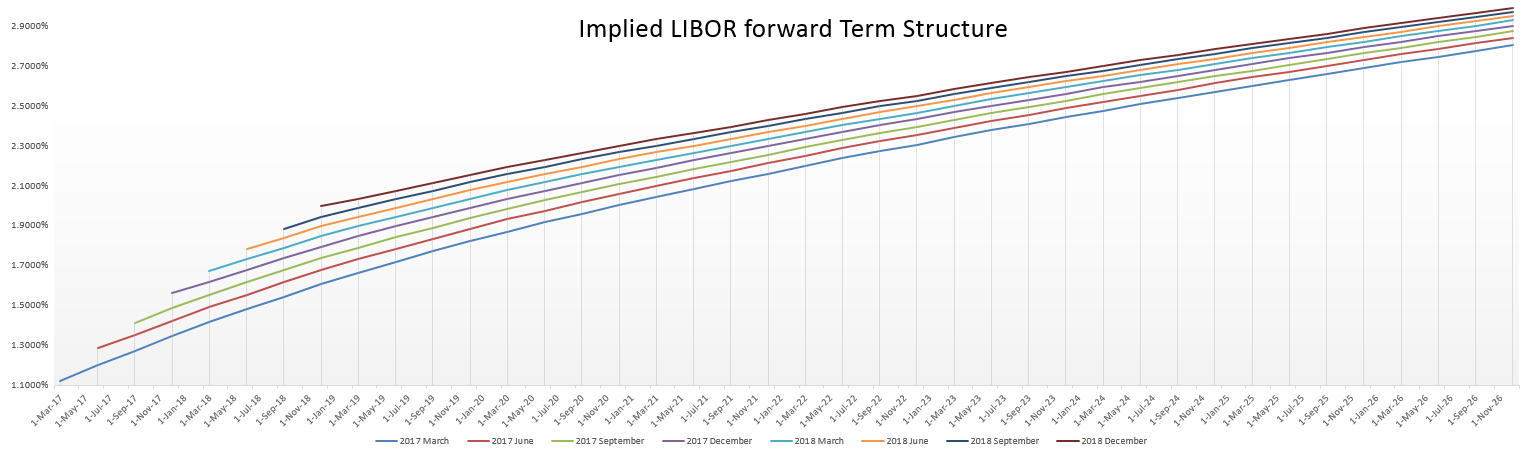
\includegraphics[scale=0.5]{biu.PNG}
	\caption{$\sigma-\bar{r}$ diagram of 100 points}
\end{figure}
\\[4mm]Also, since it may be difficult to directly observe the efficient frontier from only 25 points, I have plotted a $\sigma-\bar{r}$ diagram with 100 points on the efficient frontier by incrementing $\lambda$ at 0.01 only. From the diagram with more points from the efficient frontier, we can see that the slope of the frontier decreases at a decreasing rate, and eventually becomes one straight line. This shows the existence of asymptote of the efficient frontier.
\end{document}